%Conclusion body
%Created SS 04-14

\section{Results}
\label{results}

\subsection{Second Sound Results}
\label{secondsoundresults}

To measure the velocity of second sound in He-II.  

First the displacement between the thermometer (better name) and the heater (both fully submerged) was measured. Next, a heat pulse was sent from the heater which then propagated towards the thermometer as second sound.  The duration between the triggering of the heat pulse and the pulse's signature recorded by the thermometer was observed and recorded.


\begin{figure}[htbp]
\begin{center}
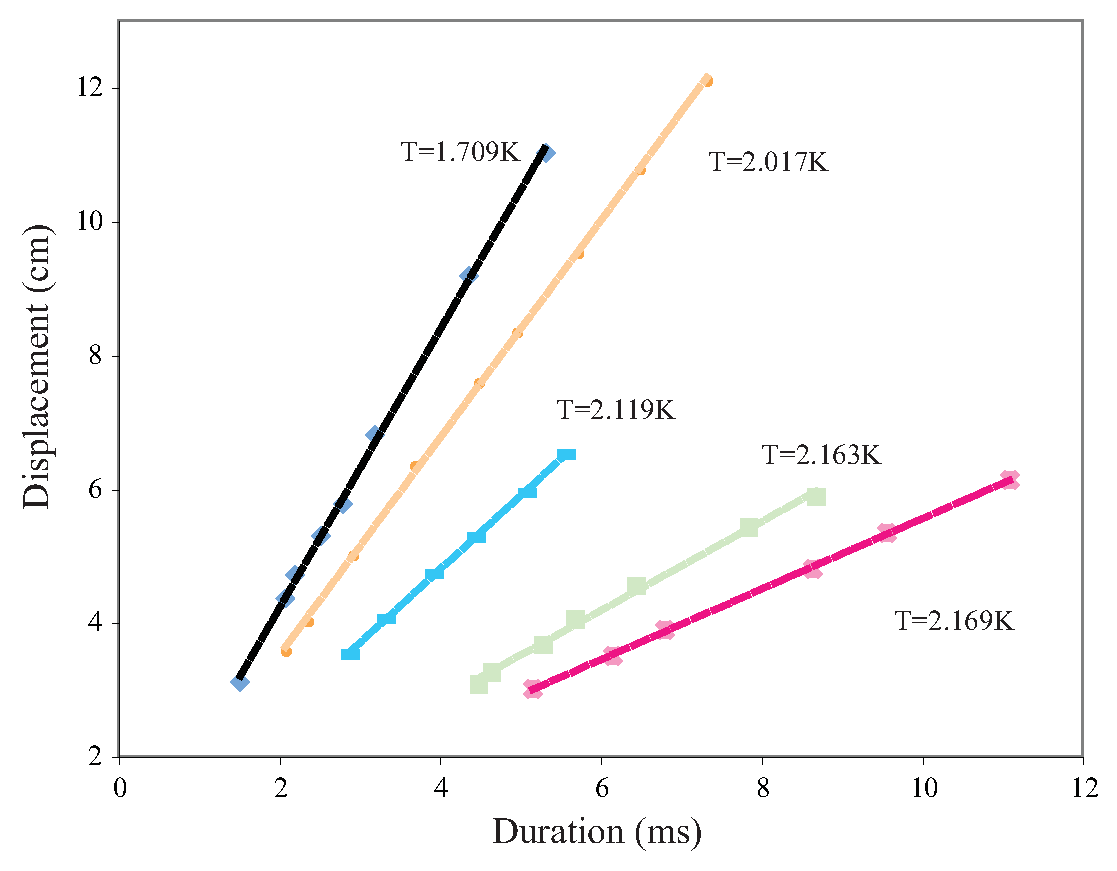
\includegraphics[height=70mm]{./figures/secondsoundraw.eps}
\caption{\small{A plot of the displacement of the thermometer from the heater verses the duration between the triggering of the heat pulse and the pulse's signature recorded by the thermometer for various temperatures in He (II).}}
\label{fig:secondsoundraw}
\end{center}
\end{figure}


\subsection{Heat Capacity Results}\label{heatcapacityresults}

\begin{figure}[htbp]
\begin{center}
\subfigure[Cu Addendum]{\label{fig:edge-a}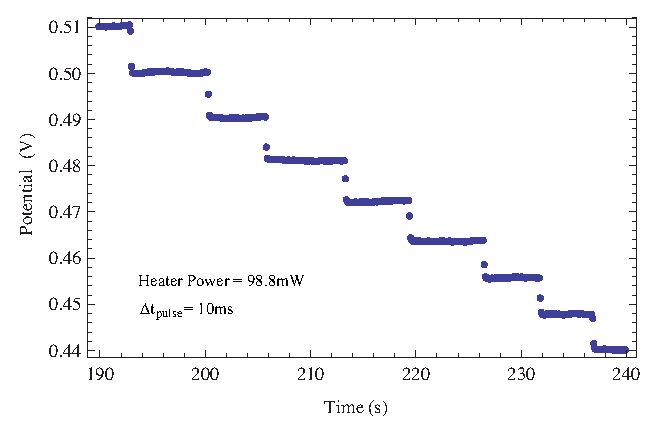
\includegraphics[height=52mm]{figures/rawcu.eps}}
\hspace{-1mm}
\vspace{-2mm}
\subfigure[He (II) and Cu Addendum near $T_{\lambda}$]{\label{fig:edge-b}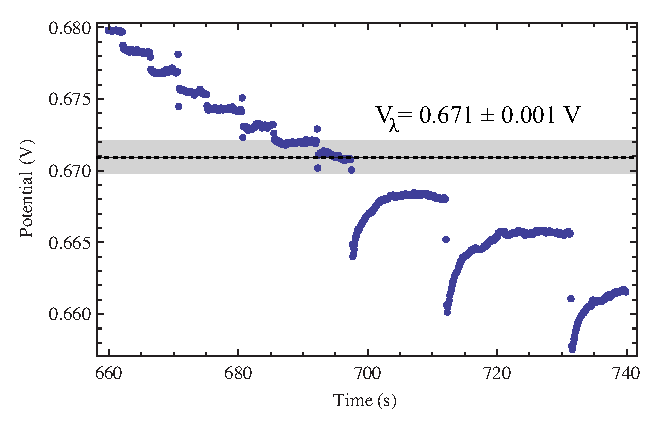
\includegraphics[height=52mm]{figures/rawhe.eps}}
\vspace{-2mm}
\caption{\small{Plots showing the change in the thermometer's potential difference due to heat pulses sent to (a) the evacuated addendum and (b) the addendum filled with He(II).  Each heat pulse is $10$ ms with a power of $98.8$ mW.  From this data we see that $T_{\lambda}$ occurs at $0.671 \pm 0.001$ V judging by the sudden change of the heat pulse's signature.}}
\label{fig:rawdata}
\end{center}
\end{figure}